\documentclass{ucph-handout}
%\usepackage[english]{babel}
\usepackage[utf8]{inputenc}
\usepackage{listings}
\usepackage{xcolor}
\usepackage{hyperref}
\usepackage{wrapfig}
\newcounter{handout}
\newcommand{\Ark}{Worksheet \arabic{handout}: }
\renewcommand{\Title}{\Ark Kickstart 2025 P5js}%
\renewcommand{\TimeAndLocation}{DIKU, 2025}%
\renewcommand{\Author}{Daniel Spikol \& Martin Dybdal}
\renewcommand{\AuthorEmail}{ds@di.ku.dk}
% Define JavaScript language settings for listings
\lstdefinelanguage{JavaScript}{
  keywords={typeof, new, true, false, catch, function, return, null, catch, switch, var, if, in, while, do, else, case, break},
  keywordstyle=\color{blue}\bfseries,
  ndkeywords={class, export, boolean, throw, implements, import, this},
  ndkeywordstyle=\color{darkgray}\bfseries,
  identifierstyle=\color{black},
  sensitive=false,
  comment=[l]{//},
  morecomment=[s]{/*}{*/},
  commentstyle=\color{purple}\ttfamily,
  stringstyle=\color{red}\ttfamily,
  morestring=[b]',
  morestring=[b]"
}
\begin{document}
\begin{exercisebox}[adjusted title=Welcome to Kickstart]
Welcome to Computer Science and the programming kickstart course!
The exercises below will quickly get you up and running with programming P5 JavaScript. We have intentionally left some things unexplained as we want you to want you to experiment on your own.
\end{exercisebox}
\begin{exercisebox}[adjusted title=Resources]
There is a world of information and resources to help you learn p5.js. Check out the following:
\begin{description}
\item[Book] McCarthy, Lauren, Casey Reas, and Ben Fry. Getting started with P5. js: Making interactive graphics in JavaScript and processing. Maker Media, Inc., 2015.
\item[p5.js Web site] \href{https://p5js.org/}{The official website}
\item[Happy Coding] A fun set of tutorials and examples for p5.js: \href{https://happycoding.io/}{Happy Coding}
\item[Kickstart Absalon] You can find the book and other materials on the LMS.
\end{description}
\end{exercisebox}
\begin{exercisebox}[adjusted title=Have Fun]
\begin{center}
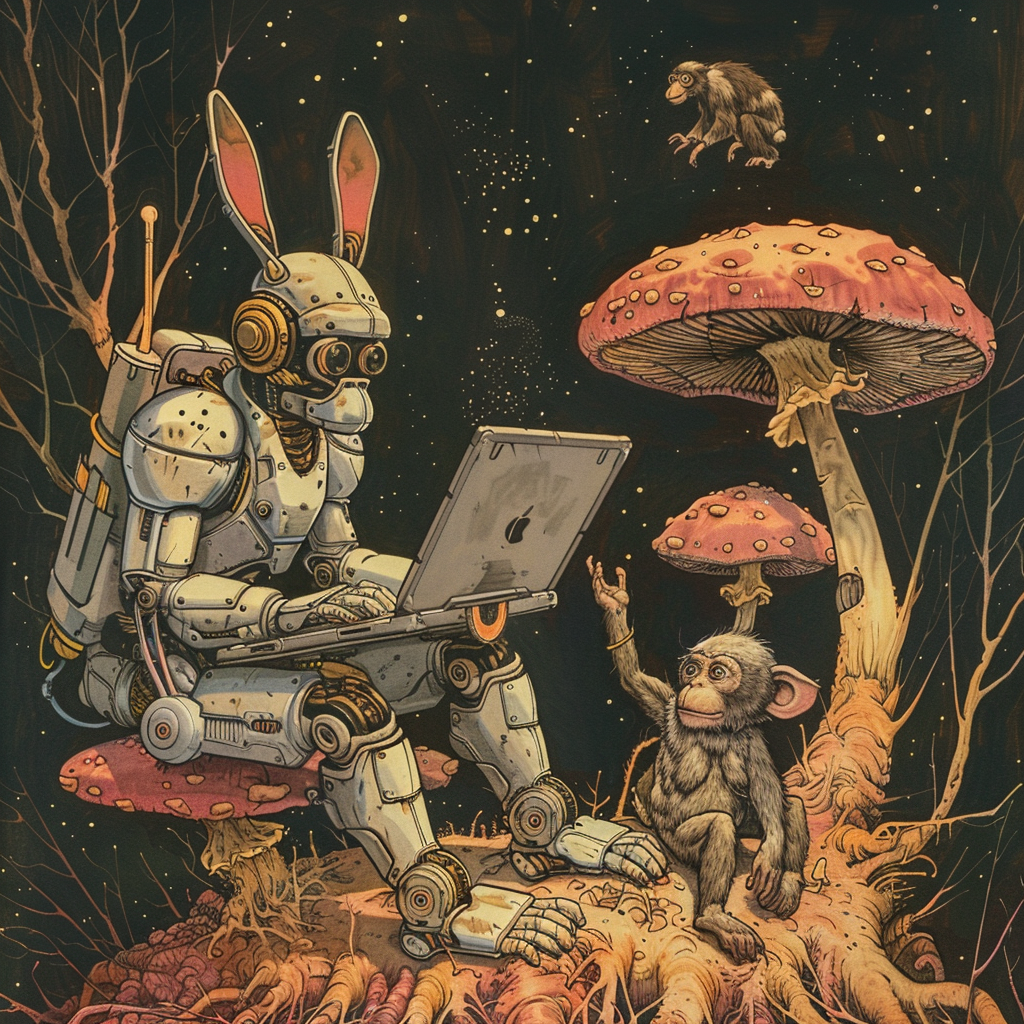
\includegraphics[width=0.5\textwidth]{illustrationer/monkey_fun.png}
\end{center}
\end{exercisebox}
%==WORKSHEET 1
%==WORKHEET 1
\newpage
\stepcounter{handout}
\begin{exercisebox}[adjusted title=First Program]
Type the following example in the Processing editor and press

\includegraphics[height=4mm]{illustrationer/processing_play_button}-button:

\begin{lstlisting}[language=JavaScript]
function setup() {
  //set the canvas and background color
  createCanvas(400, 400);
  background(220);
  
  // Tree
  rect(55, 50, 10, 20);
  ellipse(60, 35, 30, 40);
}

function draw() {}


\end{lstlisting}


Then add the following into the setup() function:
\begin{lstlisting}[language=JavaScript]
  // powerplant
  rect(120, 50, 60, 30);
  rect(160, 20, 10, 30);
  triangle(120, 50, 136, 40, 136, 50);
  triangle(136, 50, 152, 40, 152, 50);

\end{lstlisting}
And:
% \begin{python}
% # Person
% ellipse(270, 65, 8, 8)
% line(270, 70, 270, 75)
% line(270, 69, 277, 75)
% line(270, 69, 263, 75)
% line(270, 75, 275, 82)
% line(270, 75, 265, 82)
% \end{python}
\begin{lstlisting}[language=JavaScript]
  // windmill
  line(300, 50, 320, 51);
  line(300, 50, 289, 67);
  line(300, 50, 291, 32);
  line(300, 50, 300, 90);
\end{lstlisting}

\tcbsubtitle{Now try drawing a car and a cloud:}
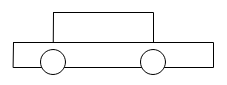
\includegraphics[width=0.4\textwidth]{illustrationer/bil-streg.png}
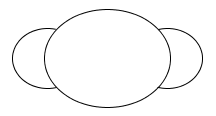
\includegraphics[width=0.3\textwidth]{illustrationer/sky.png}
\end{exercisebox}

\begin{exercisebox}[adjusted title=Colors]
You are now going to colour the shapes. To do this, use the
\ttpy{fill(r, g, b)} function, which selects which colour 
to use for fill and text colour. It's all about calling
\ttpy{fill} in the right places! As arguments, you specify the amount
of red (0-255), blue (0-255), and green (0-255).
\noindent
Here are some basic colors to experiment with:
\begin{minipage}{0.45\linewidth}
\begin{lstlisting}[language=JavaScript]
fill(255, 0, 0);  // red
fill(0, 255, 0);  // green
fill(0, 0, 255);  // blue
\end{lstlisting}
\end{minipage}
\begin{minipage}{0.45\linewidth}
\begin{lstlisting}[language=JavaScript]
fill(0, 0, 0);       // black
fill(255, 255, 255); // white
fill(255, 255, 0);   // yellow
\end{lstlisting}
\end{minipage}

\noindent
Optionally, find colours using an online color picker or RGB
colour table. For example, search for ``RGB color picker''.
\tcbsubtitle{Lines and outlines}
To specify the colour of strokes (e.g. \ttpy{line}) and outlines, use \ttpy{stroke(r, g, b)}. Also try the \ttpy{noStroke()} function, to turn off outline drawing.
\end{exercisebox}

\begin{exercisebox}[adjusted title=Example]
\noindent
Here's an example of what it might look like after colouring:
\begin{center}
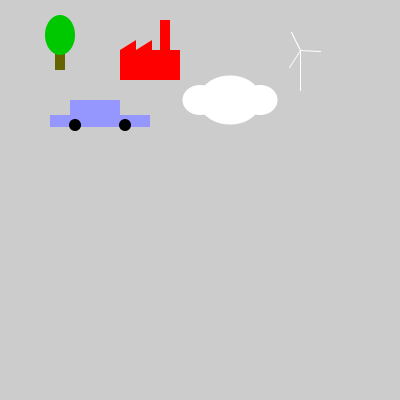
\includegraphics[width=0.5\textwidth]{illustrationer/farvelagt.png}
\end{center}
\end{exercisebox}

\begin{exercisebox}[adjusted title=Green City]
%Gem projektet og giv det navnet ``Elbil''. Senere skal vi udbygge dettil en simulation hvor bilen skal lades med strøm fra enten vindmølleeller kraftværket, men hvor bilen helst skal lades op med grøn strøm fra vindmøllen.

Use what you've learned to make it a slightly nicer scene, with background, foreground and the extra details you think should be there. For example, I've drawn a road and moved the characters around. 
\\
\\
\textbf{Tip: }To change the background color from gray you can use \ttpy{rect} which you
already know, but you can also use the \ttpy{background(r, g, b)} command.
It will delete everything and fill the screen with the specified colour.

\begin{center}
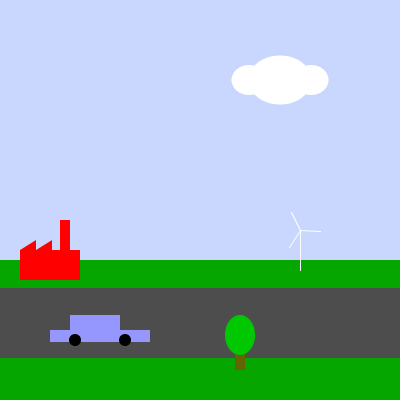
\includegraphics[width=0.5\textwidth]{illustrationer/elbil.png}
\end{center}

\noindent
Remember to use comments to find your way around the code easily!
Commenting code is good because it improves code readability and maintainability by explaining the purpose and functionality of the code to others and to your future self.



\end{exercisebox}

%==WORKSHEET 2
%==WORKSHEET 2

\newpage
\stepcounter{handout}
\begin{exercisebox}[adjusted title=Variables]
Create a new project (``File'' -> ``New'') and immediately save it
the project. Call it ``Aquarium''.\\
\\
\noindent
Type in this piece of code:

\begin{lstlisting}[language=JavaScript]
function setup() {
  createCanvas(400, 400);
  background(220);
  
  //basic fish shape
  fishX = 150;
  ellipse(fishX, 200, 120, 75);
  triangle(fishX - 60, 200, fishX - 90, 170, fishX - 90, 230);
}

function draw() {
 
}

\end{lstlisting}
Try changing 150 to a different number in the \ttpy{fishX} specification.

\noindent
Now add the following:
\begin{lstlisting}[language=JavaScript]
  eyeSize = 15;
  ellipse(fishX + 30, 190, eyeSize, eyeSize);
\end{lstlisting}
Try changing the value of \ttpy{eyeSize}.

\tcbsubtitle{Tasks:}
\noindent
You have now added a fish that can be moved just by changing one
value.

\begin{itemize}
\item Color the fish
\item Give the fish a fin that moves when you change \ttpy{fishX}.
\item Give the fish a pupil that moves when you change \ttpy{fishX}.
\item Create a new variable, \ttpy{fishY}, that controls the y-position of the fish
\end{itemize}

\hspace{1cm}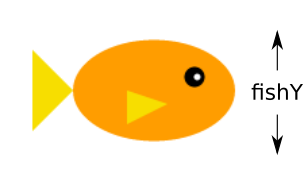
\includegraphics[width=0.4\textwidth]{illustrationer/fisk-fishY.png}

\noindent
Remember to save the project. We'll be working on it later.

\end{exercisebox}
\newpage
\begin{exercisebox}[adjusted title= Green City continues]
Switch to the electric car project and introduce variables to specify the
location of the objects so that we can later animate these objects.

\begin{itemize}
\item Create a variable \ttpy{carX} so the car can move forward
  and back
\item Create a variable \ttpy{cloudX} so the cloud can move back and forth
\item Create a variable \ttpy{treeX} so the tree can be moved horizontally
\item Create a variable \ttpy{treeY} so the tree can be moved vertically
\end{itemize}
\begin{center}
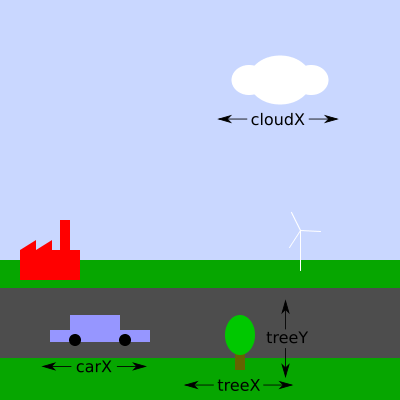
\includegraphics[width=0.5\textwidth]{illustrationer/carX-cloudX-treeXY.png}
\end{center}
\end{exercisebox}

\begin{exercisebox}[adjusted title=Aquarium Continues]
Use what you've learned to expand your aquarium project; here's an
example, but feel free to use your imagination! For example, one variable is used
for the x-coordinate of the seaweed plant and another variable for the x-coordinate
of the entire group of rocks (as a unit). An additional set of
variables \ttpy{fish2X}/\ttpy{fish2Y} to control the location of the
additional fish.%  Man kunne også forestille sig bobler, et mini sandslot,
% andre tangplanter, muslingeskaler eller andre dyr.

\begin{center}
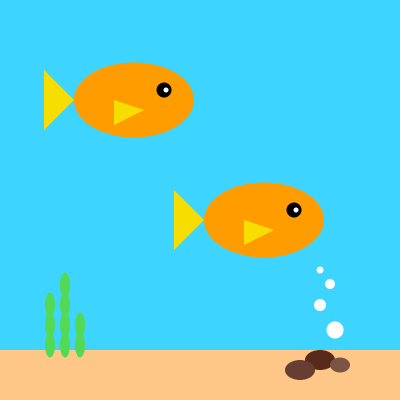
\includegraphics[width=0.4\textwidth]{illustrationer/akvarie.png}
\end{center}

\end{exercisebox}

%==WORKSHEET 3

%==WORKSHEET 3
\newpage
\stepcounter{handout}

\begin{exercisebox}[adjusted title=Functions]
Functions allow you to reuse the same code in multiple places,
name entire blocks, and add structure to code.\\

Open the Aquarium project. Add the following ``fish-draw-function'':

\begin{lstlisting}[language=JavaScript]
function setup() {
  // Set up the canvas
  createCanvas(400, 400);
  
  // Set the background color to light grey
  background(220);
}

function draw() {
  // Draw the first fish at x-coordinate 100
  make_fish(100);
  
  // Draw the second fish at x-coordinate 280
  make_fish(280);
}

function make_fish(fishX) {
  // Draw the basic fish shape
  // Draw fish body  (fishX, 200) with a width of 120 and height of 75
  ellipse(fishX, 200, 120, 75);
  
  // Draw the fish tail using a triangle
  // The triangle points are at (fishX - 60, 200), (fishX - 90, 170), 
  //and (fishX - 90, 230)
  triangle(fishX - 60, 200, fishX - 90, 170, fishX - 90, 230);

  // Draw the fish eye
  // The eye is a small ellipse located at (fishX + 30, 190) 
  //with a size of 15x15
  eyeSize = 15;
  ellipse(fishX + 30, 190, eyeSize, eyeSize);
}

\end{lstlisting}

Now it's much faster to fill the aquarium with fish and we avoid copying code.

\tcbsubtitle{Task:} Create your own \texttt{drawFish(x, y)} function that draws your entire fish with colour, fins and eyes.

\end{exercisebox}

\begin{exercisebox}[adjusted title=Notes and Extra]
\begin{itemize}
\item Try changing $50$ to another number
\item Try changing the line \ttpy{x = x + 1} to \ttpy{x = x - 1} or to \ttpy{x = x + 5}
\item Try moving the call to \ttpy{background} from \ttpy{draw}
 to \ttpy{setup} - what happens?
\end{itemize}

\end{exercisebox}

\begin{exercisebox}[adjusted title=BE AWARE]

When using setup/draw, call draw functions outside of setup
and draw are not allowed. Everything must be moved into the two functions.

\end{exercisebox}


\begin{exercisebox}[adjusted title=Green City continued]
Over in the electric car project, you can also try writing a function
to draw trees:
\begin{lstlisting}[language=JavaScript]
 function setup() {
  createCanvas(400, 400);
  background(220);
  drawTree(160);
}

function draw() {
  // we are going to use the draw function soon!
}

function drawTree(treeX) {
  fill(100, 100, 0);
  rect(treeX - 5, 350, 10, 20);
  fill(0, 200, 0);
  ellipse(treeX, 335, 40, 50);
}
\end{lstlisting}

\noindent
Structure your electric car project code with functions:
\begin{itemize}
\item Write a \texttt{drawCloud(x)} function that draws a cloud
\item Extend the \texttt{drawTree(x)} function to also accept a y-coordinate
\item Write a \texttt{drawCar(x)} function that draws a car
\item Write a \texttt{drawPowerplant()} function and a
  \texttt{drawWindmill()} function that draws the power plant and
  the windmill, respectively. We won't need to move them around, so they don't need to
  not take coordinates as an argument.
\end{itemize}
\noindent
Call all the functions in the \texttt{setup() }for now. For example:

\begin{lstlisting}[language=JavaScript]
drawTree(150, 235);
drawTree(240, 335);
drawPowerplant();
drawWindmill();
drawCar(50);
drawCloud(280);
\end{lstlisting}

\end{exercisebox}

% == Worksheet 4
% == Worksheet 4A
%\newpage
%~
\newpage
\stepcounter{handout}
\begin{exercisebox}[adjusted title= Animation and Functions]% \ttpy{setup}/\ttpy{draw}]

Please create a new temporary project (you don't need to save it). Type in
this piece of code:

\begin{lstlisting}[language=JavaScript]
// declare global variable accessible from any part of the code
let globalVarX = 50;

function setup() {
  createCanvas(400, 400);
}

function draw() {
  background(220);
  background(255, 255, 255);
  fill(255, 0, 0);
  ellipse(globalVarX, 100, 30, 30);
  globalVarX = globalVarX + 1;
}

\end{lstlisting}

\noindent
The \ttpy{draw} function is automatically called 60 times per second!

\tcbsubtitle{Tasks:}
\begin{itemize}
\item Try changing  $50$ in \ttpy{globalVarX} to different number.
\item Try changing the line \ttpy{x = x + 1} to \ttpy{x = x - 1} or to \ttpy{x = x + 5}
\item Try moving the call to \ttpy{background} from \ttpy{draw}
  to \ttpy{setup} - what happens?
\end{itemize}


\tcbsubtitle{NOTE!!:}  % check this
When using
\ttpy{setup}/\ttpy{draw}~ it is not allowed to call
drawing functions outside of \ttpy{setup} and
\ttpy{draw}, everything must be moved into the two functions.

\end{exercisebox}

\begin{exercisebox}[adjusted title= Aquarium continues]
\begin{itemize}
\item \emph{Rewriting the aquarium project to use \ttpy{setup}/\ttpy{draw}:}
 \begin{itemize}
 \item Add empty \ttpy{setup} and \ttpy{draw} functions to the bottom of the program
 \item Call \ttpy{size(400, 400)} in \ttpy{setup}
 \item Call all the drawing functions in \ttpy{draw}, incl. drawing of the background
 \end{itemize}

\item \emph{Make the fish swim:}
 \begin{itemize}
 \item Create two global variables \ttpy{fish1X} and
 \ttpy{fish2X} (before \ttpy{setup}/\ttpy{draw})
 \item Use the new variables as x-argument when you call \ttpy{drawFish()}
 \item \emph{REMEMBER} the lines: ~\ttpy{global fish1X}~ and ~\ttpy{global fish2X}~
 \item Update the variables with $+1$/$-1$ inside the \ttpy{draw} function
 \end{itemize}
\end{itemize}
\end{exercisebox}

\begin{exercisebox}[adjusted title= Green City continues]

\begin{itemize}
\item Create two global variables \ttpy{carX} and \ttpy{cloudX}
\item Make the car drive to the right
\item Make the cloud start outside the image on the right side and move to the left
\end{itemize}
\end{exercisebox}


%%\emph{TODO: illustrationer}
\begin{exercisebox}[adjusted title= Randomness]
Create a brand new project and save it as ``random\_circles''. Add the following code:
\begin{minipage}{0.60\linewidth}

\begin{lstlisting}[language=JavaScript]
function setup() {
  createCanvas(400, 400);
  background(220);
}

function draw() {
  // create 2 variables for different x y coordinates on the canvas
  let x = random(0, width);
  let y = random(0, height);
  
  // color the circle with a random monochrome shade
  fill(random(255));
  
  // draw the ellipse every frame
  ellipse(x, y, 30, 30);
}

\end{lstlisting}
\end{minipage}

\begin{minipage}{0.40\linewidth}
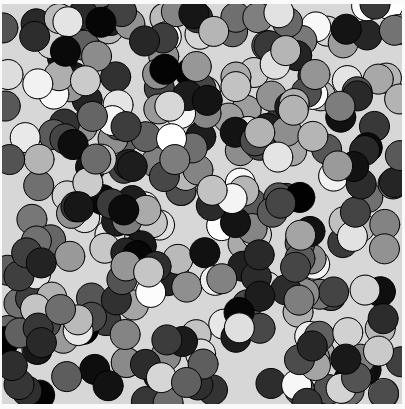
\includegraphics[width=0.70\textwidth]{illustrationer/randomcircles.png}
\end{minipage}
~
\end{exercisebox}

%\begin{minipage}{0.45\textwidth}
%\begin{Right}

%\end{Right} \end{minipage}

\begin{exercisebox}[adjusted title=Tasks: ]


\begin{itemize}
\item Make the circles change size randomly
\item Make the circles be drawn in random colours. Experiment until you find a colour scale that you think is nice.
\end{itemize}

\end{exercisebox}

\begin{exercisebox}[adjusted title=Interaction with the Mouse]
The position of the mouse can be read with the variables \ttpy{mouseX}
and \ttpy{mouseY}. A kind of drawing program can be written like this:

\begin{lstlisting}[language=JavaScript]
function setup() {
  createCanvas(800, 800);
  background(255, 204, 0);
}

function draw() {
  fill(0, 0, 0);
  ellipse(mouseX, mouseY, 5, 5);
}

\end{lstlisting}

\end{exercisebox}

\begin{exercisebox}[adjusted title=Keyboard input]
%\chapter{Tastatur input}
Open the drawing program project and try adding the following new function:

\begin{lstlisting}[language=JavaScript]
function setup() {
  createCanvas(400, 400);
  background(0);
}

function draw() {
  
}

function keyPressed(){
  background(0,0,255,255);
}
\end{lstlisting}

Start the program and press any key on the keyboard. To
check for a specific key, the variable ``\ttpy{key}'' can be read.

\begin{lstlisting}[language=JavaScript]
 if (key == 'c') { // Check if the 'c' key is pressed
    background(255, 204, 0); // Set background color to a blue hue
\end{lstlisting}
%NEED FOOTNOTE
\end{exercisebox}

\begin{exercisebox}[adjusted title=New Project:Creative Programming ]
The task is now to create a more elaborate drawing program. Sign
lines from all corners and midpoints on the sides. Use
the variables \ttpy{width} and \ttpy{height}.
\begin{center}
 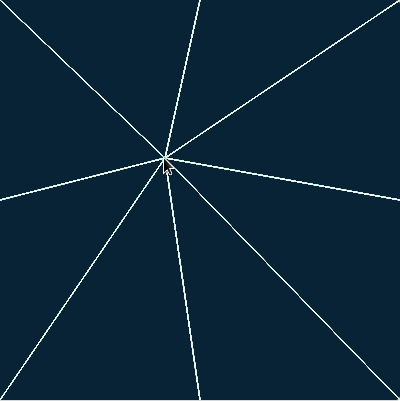
\includegraphics[width=0.40\textwidth]{illustrationer/kryds.png}
 \quad
 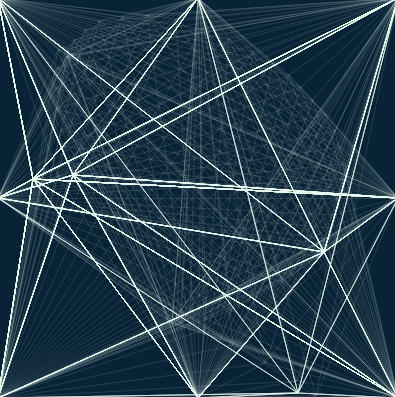
\includegraphics[width=0.40\textwidth]{illustrationer/kryds-tegning.png}
\end{center}
Remember to save the project!
\end{exercisebox}

%==WORKSHEET #5
%==WORKSHEET #5
\newpage
\stepcounter{handout}
\begin{exercisebox}[adjusted title= Conditionals]
With conditions, we can make things happen when special criteria are met
met. Open the aquarium project and try inserting the following into it
The \ttpy{draw} function:


\begin{lstlisting}[language=JavaScript]
if (fish1X > 500) {
    fish1X = -40;
  }

  if (fish2X < -50) {
    fish2X = 200;
  }
\end{lstlisting}

\noindent
What happens?
\end{exercisebox}

\begin{exercisebox}[adjusted title= Change direction]
By making a variable that contains the direction in which the fish swims, we can change the direction when it reaches the sides.

\begin{itemize}
\item Define a global variable \ttpy{fish1XVelocity} and set it to $1$
\item Change \ttpy{fish1X = fish1X + 1} to \ttpy{fish1X = fish1X + fish1XVelocity}
\item Remove the previous \ttpy{fish1X} condition
\item Add these conditions:
\end{itemize}


\begin{lstlisting}[language=JavaScript]
if (fish1X > 400){
    fish1XVelocity = -1
    }
if (fish1X < 0){
    fish1XVelocity = 1
    }
\end{lstlisting}
\end{exercisebox}

\begin{exercisebox}[adjusted title=Change appearance ]
Try changing the \ttpy{drawFish} function to strip the direction
with the fish as an argument and use a condition to draw the fins and
eyes differently depending on which direction the fish is swimming.

\begin{minipage}{0.60\linewidth}
\begin{lstlisting}[language=JavaScript]
function drawFish(x, y, eyeSize, velocity){
    ... daw body ...

    # Swim to the right
    if (velocity >= 0){
        ...draw fins and eyes ...
        }

    # Swim to the left
    if (velocity < 0){
        ...draw fins and eyes ...
        }
}
\end{lstlisting}

\end{minipage}
\begin{minipage}{0.40\linewidth}
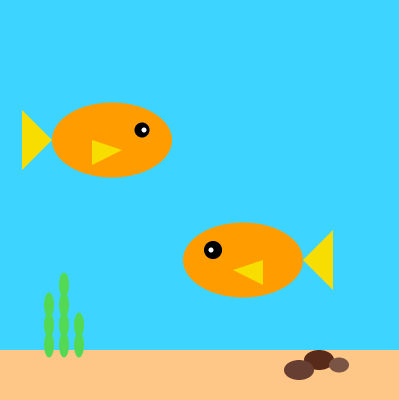
\includegraphics[width=0.70\textwidth]{illustrationer/fisk-begge-retninger.png}
\end{minipage}
~
\end{exercisebox}


\begin{exercisebox}[adjusted title=Finish the aquarium project ]
Now, we are almost done with the aquarium project. Add, if necessary, more elements. E.g. bubbles that emerge from the bottom and swim towards the surface.
\end{exercisebox}

%\newpage
%
\begin{exercisebox}[adjusted title=More exercises about conditions]
Open the Green City project and do the following:
\begin{itemize}
\item Make the cloud move back to the start and pass by again and
 again, each time it hits the edge
\item Make the car turn over at both ends.
\end{itemize}
\tcbsubtitle{Tasks:}
The car must stop when the battery is empty
 \begin{itemize}
 \item Define a global variable \ttpy{carBattery} and set it to 100
 \item Decrease it by 0.1 each time \ttpy{draw} is called
 \item Display the battery status using the \ttpy{text(string, x, y)} function.
 Remember to convert the number to a string using \ttpy{str()}.
 \item If the battery is empty (\ttpy{<= 0}) the car must stop (set velocity to 0)
 \end{itemize}
Add a \ttpy{keyPressed()} function and make it possible to charge the electric car when you press 'C':
 \begin{itemize}
 \item Add \ttpy{0.3} to \ttpy{carBattery} every time 'C' is pressed on the keyboard
 \item If \ttpy{carBattery} exceeds 100, set it to 100 so you can't charge more than 100\%
 \end{itemize}
\end{exercisebox}


\begin{exercisebox}[adjusted title= Changing wind speed]
The variable \ttpy{frameCount} counts how many times \ttpy{draw} is
run since the program started. Enter this in the draw function i
the electric car project:


\begin{lstlisting}[language=JavaScript]
fill(0, 0, 0);
text(frameCount, 350, 20):
if (frameCount % 60 == 0){
    print(frameCount)
    }
\end{lstlisting}

%new stuff


\noindent
Since \ttpy{draw} is executed at \textit{60 frames per second}, will
The \ttpy{print} function will be executed every second.

\vspace{2mm}
\noindent
We can also use that in the electric car project to update
the wind speed every second.
 \begin{itemize}
 \item Create a global windSpeed ​​variable
 \item Update windSpeed ​​with a new random value every second
 \item Display the wind speed using \ttpy{text()}
 \end{itemize}
% \item Turn the power plant on and off
 \begin{itemize}
 \item Create a global variable \ttpy{powerplantOn}
 \item Make it possible to turn the power plant on and off with a press of 'p'
 \item Draw clouds of smoke over the power plant when it is on
 \item Create a variable \ttpy{co2emission} and add a bit as long
 the power plant is on. Display the value with \ttpy{text()}
 \end{itemize}
 \end{exercisebox}


\begin{exercisebox}[adjusted title= Introduction to Sounds]
In this small worksheet, we will add sound files to make sound effects!

\begin{enumerate}
\item First check reference https://p5js.org/reference/p5.MediaElement/play/
\item Then download the sound files from ABASALON 
\item Also check out the sound sketch also uploaded
\item Create a new file and names  \ttpy{sound01}

\end{enumerate}


\begin{lstlisting}[language=JavaScript]
function preload() {
  // Load the sound files before the program starts
   // Load the first sound file (e.g., a music track or sound effect)
  sound = loadSound('sound.mp3'); 
  // Load the second sound file (e.g., a ball tap sound)
  sound1 = loadSound('balltap.wav');  
}

function setup() {
  // Setup the canvas size
  createCanvas(400, 400);  // Create a canvas of 400x400 pixels
}

function draw() {
  // Draw the background and instructions
  background(220);  // Set the background color to light grey (RGB value: 220)
  // Align text to the center horizontally and vertically
  textAlign(CENTER, CENTER);  
  textSize(24);  // Set the text size to 24 pixels
  // Display the instructions in the center of the canvas
  text('Press "S" or "A" to play sound', width / 2, height / 2);  
}

function keyPressed() {
  // Detect key presses and play the corresponding sound
  if (key === 's' || key === 'S') {
    // Play the first sound when the 'S' key is pressed (case insensitive)
    sound.play();
  }
  if (key === 'a' || key === 'A') {
    // Play the second sound when the 'A' key is pressed (case insensitive)
    sound1.play();
  }
}
\end{lstlisting}

\textbf{Descrptions}

\begin{itemize}
    \item \textbf{`preload()` function}: Loads the sound files into memory before the sketch starts. This ensures that the sounds are ready to be played when triggered.
    \item \textbf{`setup()` function}: Sets up the canvas where the sketch will be displayed, specifying its size (400x400 pixels).
    \item \textbf{`draw()` function}: Continuously runs in a loop, updating the background color and displaying the instruction text centered on the canvas.
    \item \textbf{`keyPressed()` function}: Listens for specific key presses ('S' or 'A') and plays the corresponding sound when either key is pressed.
\end{itemize}

\end{exercisebox}

%With \ttpy{for loops}, we can avoid duplicated code and iteratively perform an operation, such as drawing 3 circles on a screen.
%Start a new project and insert the following code:
%
%\begin{lstlisting}[language=JavaScript]
%// Initialize Lists
%let xs = [30, 50, 70, 90, 110, 130];
%let ys = [30, 50, 70, 90, 110, 130];
%
%function setup() {
%  createCanvas(400, 400);
%  background(0);
%}
%
%function drawCircle(x, y) {
%  noStroke();
%  bubble_R = random(256);
%  bubble_G = random(256);
%  bubble_B = random(256);
%  fill(bubble_R, bubble_G, bubble_B);
%  circle(x, y, 25);
%}
%
%function draw() {
%  for (var i = 0; i < xs.length; i++) {
%    drawCircle(xs[i], ys[i]);
%  }
%}
%\end{lstlisting}
%
%What happens when you run the code? Explain here how a loop produces the result, and give yourself time to understand the logic.
%
%\end{exercisebox}
%
%\begin{exercisebox}[adjusted title= More with Lists and For Loops]
%The following code snippet has a few changes: We now use a loop to generate our list! Paste the code into a new project and consider the differences in the various loops.
%
%\begin{lstlisting}[language=JavaScript]
%// Initialize Lists
%let circleList = [];
%
%function setup() {
%  createCanvas(400, 400);
%  background(0);
%}
%
%function drawCircle(x, y) {
%  stroke(255, 255, 255);
%  noStroke();
%  bubble_R =random(255);
%  bubble_G =random(255);
%  bubble_B =random(255);
%  fill(bubble_R, bubble_G, bubble_B);
%  circle(x, 200, 50);
%}
%
%function createCircleList(n) {
%  for (var i=0; i < n; i++) {
%    append(circleList, i*60);
%  }
%}
%
%function draw() {
%  createCircleList(10);
%  for (var i = 0; i < circleList.length; i++) {
%    drawCircle(i);
%  }
%}
%\end{lstlisting}
%
%\noindent
%
%\vspace{2mm}
%\noindent
%
%\begin{itemize}
%  \item Use loops and lists to move your fish or make more fish in different locations. Plus in Green City if you want.
%\end{itemize}
%\end{exercisebox}
%=== Worksheet 06
\newpage
\stepcounter{handout}

\begin{exercisebox}[adjusted title= Introduction to Lists and For Loops]
With \ttpy{for loops}, we can avoid duplicated code and iteratively operate, such as drawing 3 circles on a screen.
Start a new project and insert the following code:

\begin{lstlisting}[language=JavaScript]
// Initialize Lists

// List of x-coordinates for the circles
let xs = [30, 50, 70, 90, 110, 130];
// List of y-coordinates for the circles
let ys = [30, 50, 70, 90, 110, 130];

function setup() {
  // Create a canvas with a width and height of 400 pixels
  createCanvas(400, 400);
  // Set the background color to black
  background(0);
}

function drawCircle(x, y) {
  // Disable the outline (stroke) for the circles
  noStroke();
  // Generate a random red color value between 0 and 255
  bubble_R = random(256);
  // Generate a random green color value between 0 and 255
  bubble_G = random(256);
  // Generate a random blue color value between 0 and 255
  bubble_B = random(256);
  // Set the fill color using the random RGB values
  fill(bubble_R, bubble_G, bubble_B);
  // Draw a circle at the specified (x, y) coordinates
  circle(x, y, 25);
}

function draw() {
  // Call the drawCircle function for each pair of (x, y) coordinates
  for (var i = 0; i < xs.length; i++) {
    drawCircle(xs[i], ys[i]);
  }
}
\end{lstlisting}
\end{exercisebox}

\begin{exercisebox}[adjusted title= Explanation Loops I ]
What happens when you run the code? Explain here how a loop produces the result, and give yourself time to understand the logic. This code draws multiple circles on a black background at predefined positions. Each circle is filled with a random color, and the process repeats every frame (due to the \texttt{draw()} function), although the positions and colors remain constant unless the \texttt{xs} or \texttt{ys} arrays are changed dynamically during execution.

\begin{enumerate}
    \item \textbf{Global Variables:}
    \begin{itemize}
        \item \texttt{xs} and \texttt{ys} are arrays (lists) that store the x and y coordinates for the circles. Each pair of values from these arrays will be used to draw a circle on the canvas.
    \end{itemize}

    \item \textbf{setup() Function:}
    \begin{itemize}
        \item The \texttt{setup()} function is called once when the program starts. It creates a canvas of 400x400 pixels and sets the background color to black.
    \end{itemize}

    \item \textbf{drawCircle(x, y) Function:}
    \begin{itemize}
        \item This is a custom function designed to draw a single circle at the specified (x, y) coordinates.
        \item Inside this function:
        \begin{itemize}
            \item \texttt{noStroke()} is called to ensure the circles don't have an outline.
            \item \texttt{random(256)} is used to generate random values for the red (\texttt{bubble\_R}), green (\texttt{bubble\_G}), and blue (\texttt{bubble\_B}) color components, resulting in a random color.
            \item \texttt{fill(bubble\_R, bubble\_G, bubble\_B)} sets the fill color for the circle using the randomly generated RGB values.
            \item \texttt{circle(x, y, 25)} draws a circle at the specified coordinates with a diameter of 25 pixels.
        \end{itemize}
    \end{itemize}

    \item \textbf{draw() Function:}
    \begin{itemize}
        \item The \texttt{draw()} function is called repeatedly, continuously executing the code within it.
        \item Inside \texttt{draw()}, a \texttt{for} loop iterates over the \texttt{xs} array. For each iteration, it retrieves the corresponding x and y coordinates from \texttt{xs} and \texttt{ys} arrays and passes them to the \texttt{drawCircle()} function to draw a circle.
        \item As a result, a set of circles is drawn on the canvas at the specified coordinates, each with a random color.
    \end{itemize}
\end{enumerate}
\end{exercisebox}






\begin{exercisebox}[adjusted title= More with Lists and For Loops II]
The following code snippet has a few changes: We now use a loop to generate our list! Paste the code into a new project and consider the differences in the various loops.

\begin{lstlisting}[language=JavaScript]
// Initialize Lists
// Empty array to hold x-coordinates for the circles
let circleList = []; 

function setup() {
  createCanvas(400, 400);  
  background(0); 
}

function drawCircle(x, y) {
  noStroke(); 
  // Generate a random  colors value between 0 and 255
  bubble_R = random(255);  
  bubble_G = random(255); 
  bubble_B = random(255);
   // Set the fill color using the random RGB values
  fill(bubble_R, bubble_G, bubble_B); 
  circle(x, 200, 50);  // Draw a circle
}

function createCircleList(n) {
// Add a new x-coordinate to the circleList array, spaced by 60 pixels
  for (var i = 0; i < n; i++) {
    append(circleList, i * 60);    }
}

function draw() {
// Draw a circle at each x-coordinate in the circleList, with y fixed at 200
  createCircleList(10);  // Populate the circleList with 10 x-coordinates
  for (var i = 0; i < circleList.length; i++) {
    drawCircle(circleList[i], 200);  
  }
}
\end{lstlisting}

\noindent


\noindent
\end{exercisebox}


\begin{exercisebox}[adjusted title= Explanation for Loops II]
\begin{itemize}
  \item \textbf{createCircleList(n) Function:}
 
  \begin{itemize}
  \item A loop runs n times, appending new values to circleList.
  \item Each value added is i * 60, where i is the loop counter, resulting in x-coordinates spaced 60 pixels apart.
		
  \end{itemize}
  \item \textbf{draw() Function:}
  \begin{itemize}
  \item createCircleList(10): Calls the createCircleList() function to generate 10 x-coordinates and store them in circleList.
\item	 A loop then iterates over circleList, calling drawCircle() for each x-coordinate, with the y-coordinate fixed at 200 pixels.
\item This results in 10 circles being drawn on the canvas.
  \end{itemize}
  \end{itemize}
\end{exercisebox}

%%%% FSM
%\begin{exercisebox}[adjusted title= Finite state machines]
%
%\begin{minipage}{1.0\linewidth}
%\begin{wrapfigure}[9]{r}{0.15\textwidth}
%   \vspace{-1em}
%   
\includegraphics[width=0.15\textwidth]{illustrationer/unitek_kombinationslaas.jpg}
%\end{wrapfigure}
% 
%As the first example of a state machine, we will create one
%electronic combination lock, such as those used for access control
%doors.
%
%\noindent
%Tilstandsdiagram:
%
%\noindent
%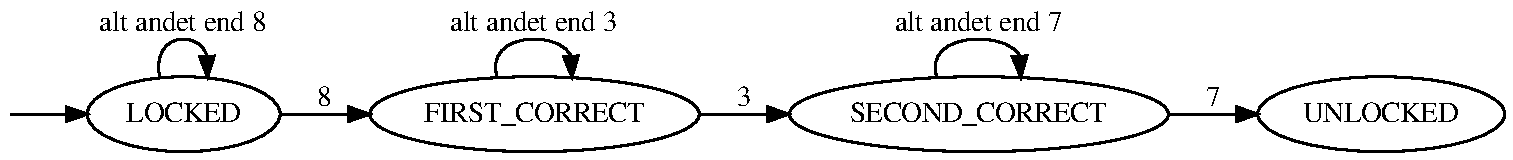
\includegraphics[width=0.85\textwidth]{graphviz/combinationLock_dumb}
%
%%%% FIX!!!!
%Download the Processing.py code for the combination lock here:
%\mbox{\url{http://kortlink.dk/ufdh}} and copy it into a new Processing project.
%
%\end{minipage}
%
%\begin{itemize}
%\item Test the combination lock and watch as the state changes. If you
%did not know the ransom (password), how many attempts does it require?
%to guess?
%
%\item Change the code so that the default is 524 instead
%\item Try changing the code to follow this diagram instead, where incorrect presses reset the state to start:
% 
%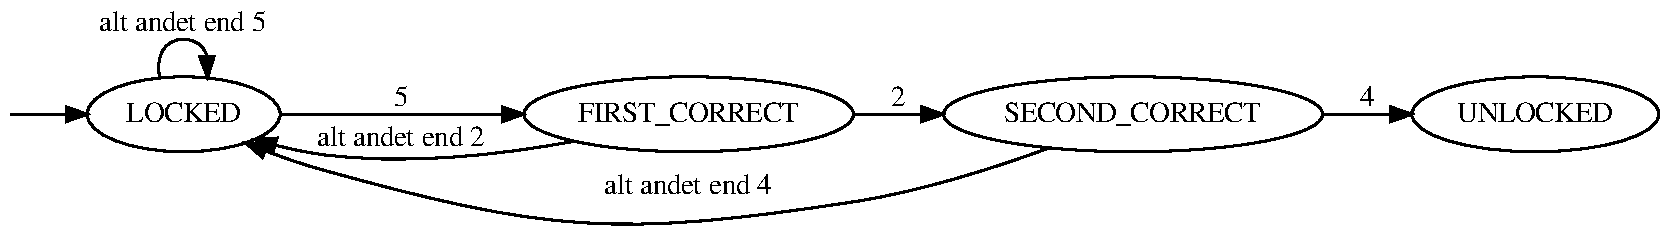
\includegraphics[width=0.85\textwidth]{graphviz/combinationLock_resetting}
%
%\item Draw an extended state diagram of the combination lock with an extra mode, so 4 digits are required. Next, add the extra state in the code.
%\end{itemize}
%\end{exercisebox}
%
%\begin{exercisebox}[adjusted title= Automatic relock after 2 seconds]
%
%Let's extend the lock so that the door automatically locks again after 2 seconds,
%which corresponds to 120 frames:
%
%\noindent
%\begin{center}
%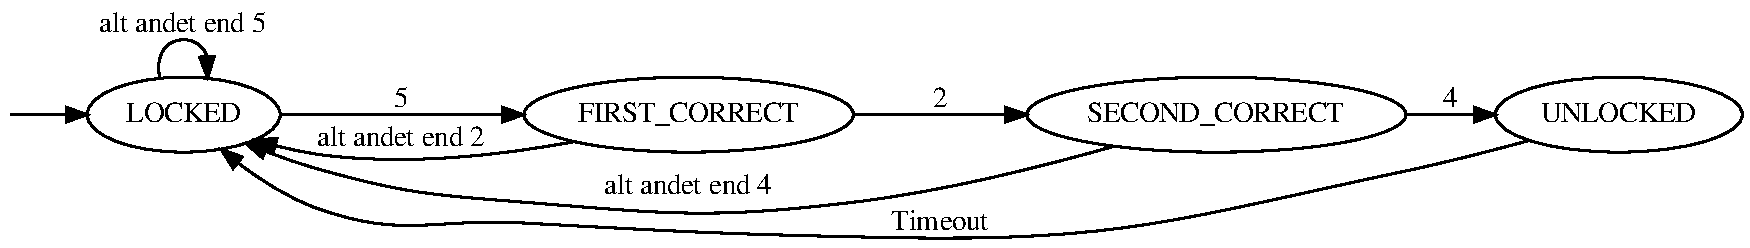
\includegraphics[width=1.0\textwidth]{graphviz/combinationLock_timeout}
%\end{center}
%
%\begin{itemize}
%\item Create a global variable ``\ttpy{timer}'' and set it to 0
%\item Set the \ttpy{timer} variable to 120 as soon as the lock is unlocked, it will
% say when it changes \ttpy{lockState} to \ttpy{"UNLOCKED"}.
%\item Count down with the timer in each frame (add the following to the \ttpy{draw} function):
%
%
%\begin{python}
%global timer
%if timer > 0:
%   timer = timer - 1
%\end{python}
%\item Når timeren er talt helt ned, skal låsen åbnes. I
% \ttpy{draw}-funktionen skal I nu tjekke om vi er i tilstanden
% \ttpy{"UNLOCKED"} og timeren samtidig er talt ned til 0. Indsæt
% følgende i \ttpy{draw}:
% 
%\begin{python}
%if lockState == "UNLOCKED":
%   if timer == 0:
%       lockState = "LOCKED"
%\end{python}
%
%\end{itemize}
%\end{exercisebox}

%=== Worksheet 07
\include{07_worksheet}
\end{document}